%%% Template originaly created by Karol Kozioł (mail@karol-koziol.net) and modified for ShareLaTeX use

\documentclass[a4paper,11pt]{article}

\usepackage[T1]{fontenc}
\usepackage[utf8]{inputenc}
\usepackage{graphicx}
\usepackage{xcolor}

\renewcommand\familydefault{\sfdefault}
\usepackage{tgheros}
\usepackage[defaultmono]{droidmono}

\usepackage{amsmath,amssymb,amsthm,textcomp}
\usepackage{enumerate}
\usepackage{multicol}
\usepackage{tikz}
\usetikzlibrary{arrows}

\usepackage{geometry}
\geometry{total={210mm,297mm},
left=25mm,right=25mm,%
bindingoffset=0mm, top=20mm,bottom=20mm}


\linespread{1.3}

\newcommand{\linia}{\rule{\linewidth}{0.5pt}}

% custom theorems if needed
\newtheoremstyle{mytheor}
    {1ex}{1ex}{\normalfont}{0pt}{\scshape}{.}{1ex}
    {{\thmname{#1 }}{\thmnumber{#2}}{\thmnote{ (#3)}}}

\theoremstyle{mytheor}
\newtheorem{defi}{Definition}

% my own titles
\makeatletter
\renewcommand{\maketitle}{
\begin{center}
\vspace{2ex}
{\huge \textsc{\@title}}
\vspace{1ex}
\\
\linia\\
\@author \hfill \@date
\vspace{4ex}
\end{center}
}
\makeatother
%%%

% custom footers and headers
\usepackage{fancyhdr}
\pagestyle{fancy}
\lhead{}
\chead{}
\rhead{}
\lfoot{Assignment \textnumero{} 2}
\cfoot{}
\rfoot{Page \thepage}
\renewcommand{\headrulewidth}{0pt}
\renewcommand{\footrulewidth}{0pt}
%

% code listing settings
\usepackage{listings}
\lstset{
    language=Python,
    basicstyle=\ttfamily\small,
    aboveskip={1.0\baselineskip},
    belowskip={1.0\baselineskip},
    columns=fixed,
    extendedchars=true,
    breaklines=true,
    tabsize=4,
    prebreak=\raisebox{0ex}[0ex][0ex]{\ensuremath{\hookleftarrow}},
    frame=lines,
    showtabs=false,
    showspaces=false,
    showstringspaces=false,
    keywordstyle=\color[rgb]{0.627,0.126,0.941},
    commentstyle=\color[rgb]{0.133,0.545,0.133},
    stringstyle=\color[rgb]{01,0,0},
    numbers=left,
    numberstyle=\small,
    stepnumber=1,
    numbersep=10pt,
    captionpos=t,
    escapeinside={\%*}{*)}
}

\tikzstyle{arn_n} = [circle, white, font=\bfseries, draw=black, fill=black, align=center, inner sep=0pt,text width=1.5em, text centered]% black node
\tikzstyle{arn_r} = [circle, red, draw=red, align=center, inner sep=0pt,text width=1.5em, text centered, very thick]% red node
\tikzstyle{arn_x} = [rectangle, draw=black, align=center, inner sep=0pt,minimum width=0.5em, minimum height=0.5em]% NIL 'node'

%%%----------%%%----------%%%----------%%%----------%%%

\begin{document}

\title{Theoretical Assignment \textnumero{} 2}

\author{Harsh Sinha(14265), Deepak Gangwar(14208)}

\date{09/03/2017}

\maketitle

\section*{Problem 1}

The pseudo code is as follows.

\begin{lstlisting}[label={list:first},caption=Pseudo code -- Search in an Infinite Array.]
BOOL infinite_search{
isfound = FALSE;
i = 1;
s = s;
while (isfound == 0)
{
	if (A[i] == s)
		isfound = TRUE;
	else if (A[i] < s)
		i = i * 2;
	else if (A[i] > s OR A[i] == empty)
		{
			isfound = modif_bin_search (i);
			break;
		}
}
return isfound;
}
\end{lstlisting}

\begin{lstlisting}[caption=modif\_bin\_search.]
BOOL modif_bin_search (int i)
{
	L = i / 2;
	R = i;
	mid = (L + R) / 2
	while (L < R)
	{
		if (A[mid] == s)
			return TRUE;
		else if (A[mid] < s)
			L = mid + 1;
		else if (A[mid] > s OR A[mid] == empty)
			R = mid -1;	
	}
	return FALSE;
}
\end{lstlisting}

\textbf{Proof of correctness}\\
For the infinite\_search() function, in order to prove correctness we can take the assertion that if the loop breaks after i iterations then the given key must lie between i and i/2.\\
The above assertion is true for all cases irrespective the key values being found or not. Now, this function will, if the key is found, get to modified binary search. Now, for the modified binary search, we have a normal binary search only difference being, even if the value at R not be there, we are basically assuming it to be some high value. Note that this value shall always be higher than the key as that is the only case when the function is called.\\
Now this means that after ith iteration if the loop exits then they key value was lying between $k = 2^i$ and $k/2$. Now the modified binary search works the same way as a normal Binary search only except it ensures that the absence of value at k will not affect the end result.\\
Hence, this algorithm will only return correct results.
\\
\textbf{Time Complexity}\\
The function modif\_bin\_search takes log(i) steps to give us a solution (Similar to a binary search). Now the original function in the worst case takes log(n) steps. Thus in the worst possible case our algorithm shall consume 2 * log (n). Hence, the order of the given algorithm is log (n).\\
This can also be proposed by saying that the number of elements that this algorithm skips keeps on doubling every loop and so the order should be log (n).\\
Notice that the base of log (n) is decided based on our choice of the multiplier in every step.
\section*{Problem 3}
\textbf{Part (a)} Deleting 55 \\
Step I.\\
%%%%%%%%%% Step 1 %%%%%%%%%%%%%
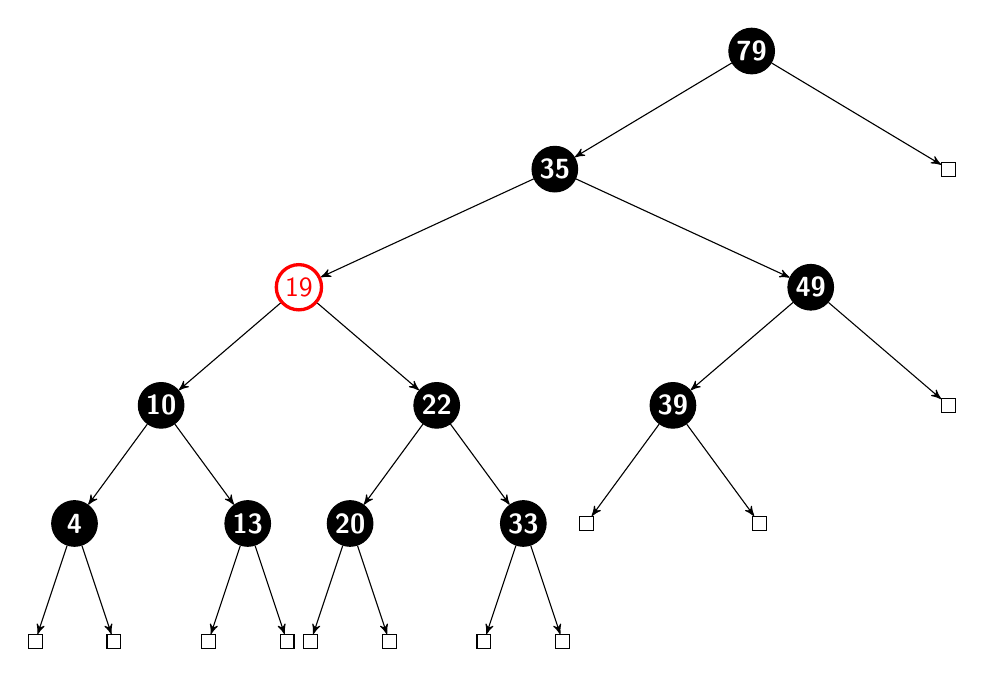
\begin{tikzpicture}[->,>=stealth',level/.style={sibling distance = 5cm/#1, level distance = 1.5cm},
level 2/.style={sibling distance = 6.5cm},
level 3/.style={sibling distance = 3.5cm},
level 4/.style={sibling distance = 2.2cm}
] 
\node [arn_n] {79}
    child{ node [arn_n] {35}
        child{ node [arn_r] {19} 
            child{ node [arn_n, name=leaf 5] {10}
            	child{ node [arn_n] {4}
					child{ node [arn_x] {}}
					child{ node [arn_x] {}}           		
            		}            	
				child{ node [arn_n] {13}
					child{ node [arn_x] {}}
					child{ node [arn_x] {}}
					}
            	}
            child{ node [arn_n] {22}
				child{ node [arn_n] {20}
					child{ node [arn_x] {}}
					child{ node [arn_x] {}}				
				}
				child{ node [arn_n] {33}
					child{ node [arn_x] {}}
					child{ node [arn_x] {}}		
					}
            	}
        	}
        child{ node [arn_n] {49}
            child{ node [arn_n] {39}
					child{ node [arn_x] {}}
					child{ node [arn_x] {}}
            }
            child{ node [arn_x] {}}
        }                            
    }
    child{ node [arn_x] {}
    }
; 
\end{tikzpicture}
%%%%%%%%%% Step 1 end %%%%%%%%%%%%%
\linebreak
\pagebreak
Step II.\\
%%%%%%%%%% Step 2 %%%%%%%%%%%%%
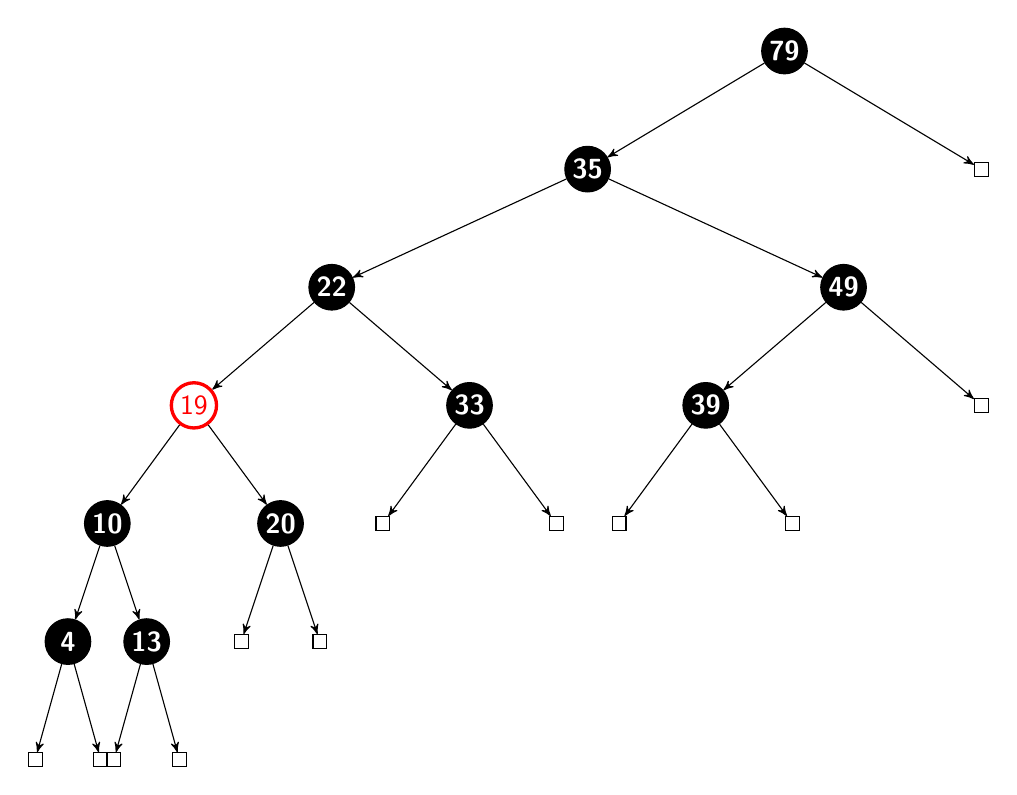
\begin{tikzpicture}[->,>=stealth',level/.style={sibling distance = 5cm/#1, level distance = 1.5cm},
level 2/.style={sibling distance = 6.5cm},
level 3/.style={sibling distance = 3.5cm},
level 4/.style={sibling distance = 2.2cm}
] 
\node [arn_n] {79}
    child{ node [arn_n] {35}
        child{ node [arn_n] {22} 
            child{ node [arn_r, name=leaf 5] {19}
            	child{ node [arn_n] {10}
					child{ node [arn_n] {4}
						child{ node [arn_x] {}}
						child{ node [arn_x] {}}					
						}
					child{ node [arn_n] {13}
						child{ node [arn_x] {}}
						child{ node [arn_x] {}}		
						}           		
            		}            	
				child{ node [arn_n] {20}
					child{ node [arn_x] {}}
					child{ node [arn_x] {}}
					}
            	}
            child{ node [arn_n] {33}
				child{ node [arn_x] {}}
				child{ node [arn_x] {}}
            	}
        	}
        child{ node [arn_n] {49}
            child{ node [arn_n] {39}
					child{ node [arn_x] {}}
					child{ node [arn_x] {}}
            }
            child{ node [arn_x] {}}
        }                            
    }
    child{ node [arn_x] {}
    }
; 
\end{tikzpicture}
%%%%%%%%%% Step 2 end %%%%%%%%%%%%%
\linebreak
Step III.\\
%%%%%%%%%% Step 3 %%%%%%%%%%%%%
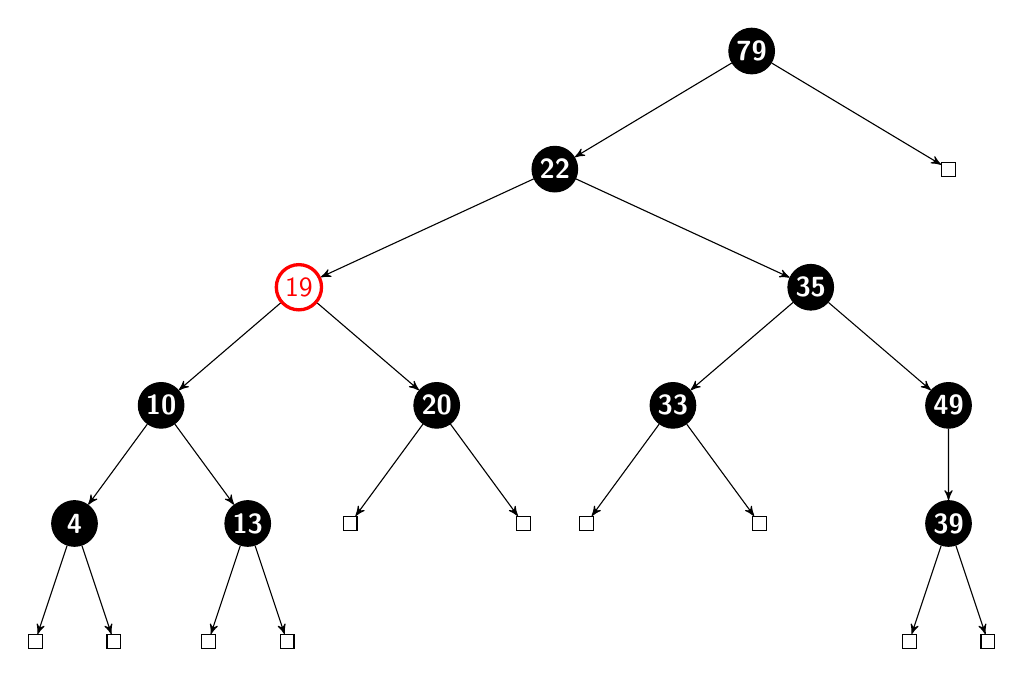
\begin{tikzpicture}[->,>=stealth',level/.style={sibling distance = 5cm/#1, level distance = 1.5cm},
level 2/.style={sibling distance = 6.5cm},
level 3/.style={sibling distance = 3.5cm},
level 4/.style={sibling distance = 2.2cm}
] 
\node [arn_n] {79}
    child{ node [arn_n] {22}
        child{ node [arn_r] {19} 
            child{ node [arn_n, name=leaf 5] {10}
            	child{ node [arn_n] {4}
						child{ node [arn_x] {}}
						child{ node [arn_x] {}}					
						}
					child{ node [arn_n] {13}
						child{ node [arn_x] {}}
						child{ node [arn_x] {}}		
						}           		
            		}            	
			child{ node [arn_n] {20}
					child{ node [arn_x] {}}
					child{ node [arn_x] {}}
					}
            	}
        child{ node [arn_n] {35}
				child{ node [arn_n] {33}
					child{ node [arn_x] {}}
					child{ node [arn_x] {}}
					}
				child{ node [arn_n] {49}
					child{ node [arn_n] {39}
						child{ node [arn_x] {}}
						child{ node [arn_x] {}}				
						}					
					}
            	}
        	}
        child{ node [arn_x] {}}                            
; 
\end{tikzpicture}
%%%%%%%%%% Step 3 end %%%%%%%%%%%%%
\linebreak
Step IV.\\
%%%%%%%%%% Step 4 %%%%%%%%%%%%%
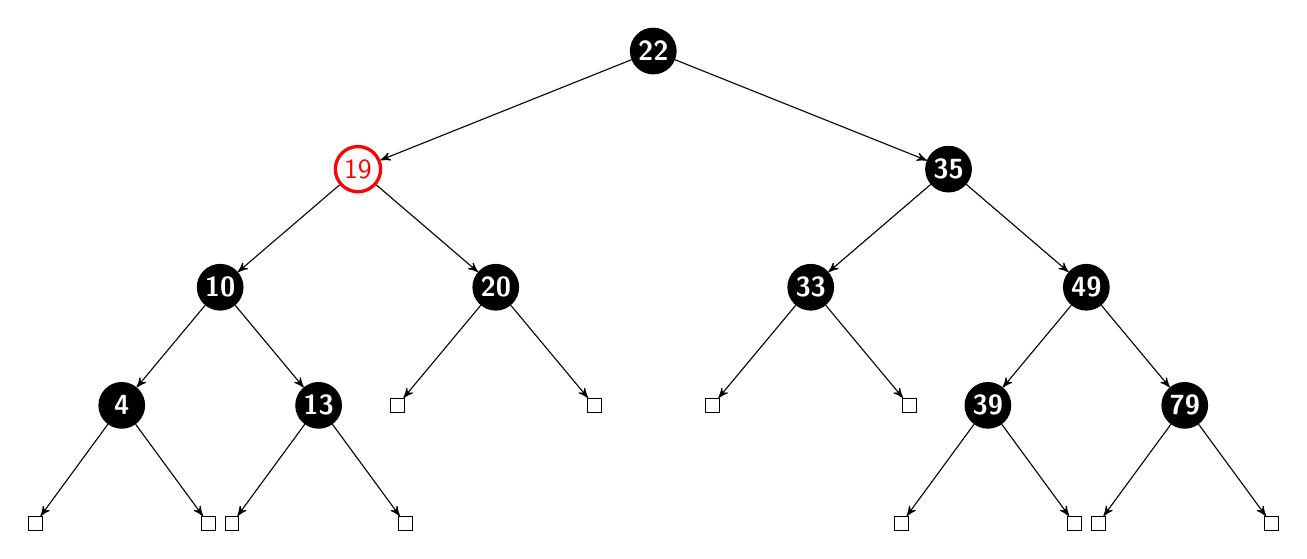
\begin{tikzpicture}[->,>=stealth',level/.style={sibling distance = 7.5cm/#1, level distance = 1.5cm},
level 2/.style={sibling distance = 3.5cm},
level 3/.style={sibling distance = 2.5cm},
level 4/.style={sibling distance = 2.2cm}
] 
\node [arn_n] {22}
        child{ node [arn_r] {19} 
            child{ node [arn_n, name=leaf 5] {10}
            	child{ node [arn_n] {4}
						child{ node [arn_x] {}}
						child{ node [arn_x] {}}					
						}
					child{ node [arn_n] {13}
						child{ node [arn_x] {}}
						child{ node [arn_x] {}}		
						}           		
            		}            	
			child{ node [arn_n] {20}
					child{ node [arn_x] {}}
					child{ node [arn_x] {}}
					}
            	}
        child{ node [arn_n] {35}
				child{ node [arn_n] {33}
					child{ node [arn_x] {}}
					child{ node [arn_x] {}}
					}
				child{ node [arn_n] {49}
					child{ node [arn_n] {39}
						child{ node [arn_x] {}}
						child{ node [arn_x] {}}				
						}					
					child{ node [arn_n] {79}
						child{ node [arn_x] {}}
						child{ node [arn_x] {}}				
						}					
					}
            	}
; 
\end{tikzpicture}
%%%%%%%%%% Step 4 end %%%%%%%%%%%%%
\linebreak
Step V.\\
%%%%%%%%%% Step 5 %%%%%%%%%%%%%
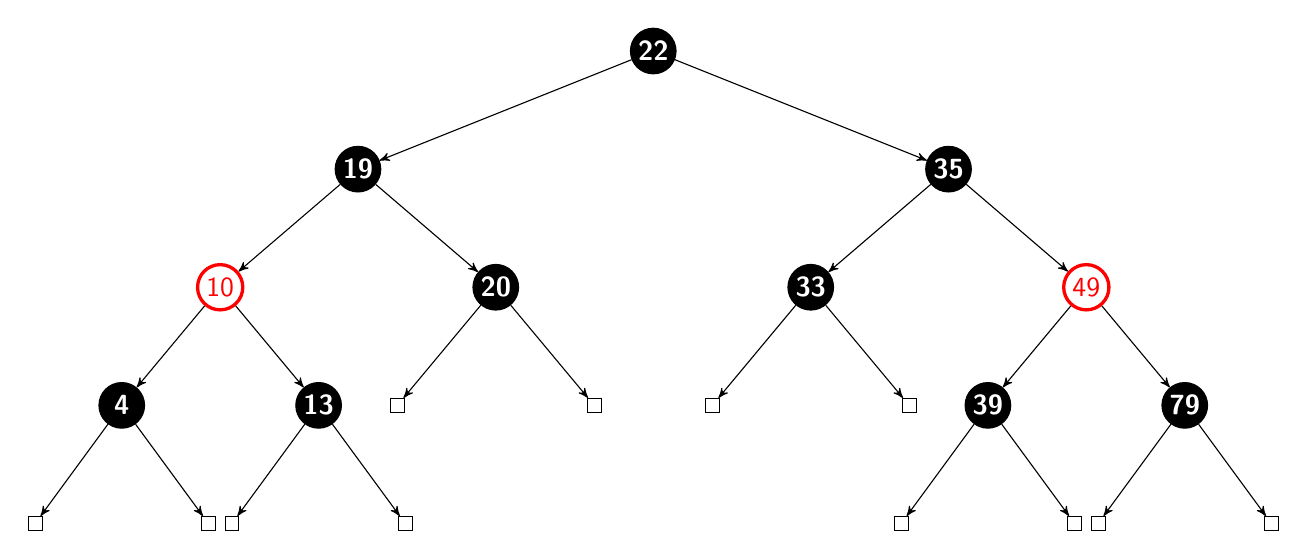
\begin{tikzpicture}[->,>=stealth',level/.style={sibling distance = 7.5cm/#1, level distance = 1.5cm},
level 2/.style={sibling distance = 3.5cm},
level 3/.style={sibling distance = 2.5cm},
level 4/.style={sibling distance = 2.2cm}
] 
\node [arn_n] {22}
        child{ node [arn_n] {19} 
            child{ node [arn_r, name=leaf 5] {10}
            	child{ node [arn_n] {4}
						child{ node [arn_x] {}}
						child{ node [arn_x] {}}					
						}
					child{ node [arn_n] {13}
						child{ node [arn_x] {}}
						child{ node [arn_x] {}}		
						}           		
            		}            	
			child{ node [arn_n] {20}
					child{ node [arn_x] {}}
					child{ node [arn_x] {}}
					}
            	}
        child{ node [arn_n] {35}
				child{ node [arn_n] {33}
					child{ node [arn_x] {}}
					child{ node [arn_x] {}}
					}
				child{ node [arn_r] {49}
					child{ node [arn_n] {39}
						child{ node [arn_x] {}}
						child{ node [arn_x] {}}				
						}					
					child{ node [arn_n] {79}
						child{ node [arn_x] {}}
						child{ node [arn_x] {}}				
						}					
					}
            	}
; 
\end{tikzpicture}
%%%%%%%%%% Step 5 end %%%%%%%%%%%%%
\linebreak
%%%%%%%%%%%%%%%%%%%Part(a)End%%%%%%%%%%%%%%%%%%%%%%%%%%%%%%%%%%%%%%%%%%%%%%%%%%%%%%%%%%%%%%%%%%%%%%%%%%%%%%%%%%%%%%%%%%%%%%%%%%%
\textbf{Part (b)} Inserting 34 \\
%%%%%%%%%% Step 1 %%%%%%%%%%%%%
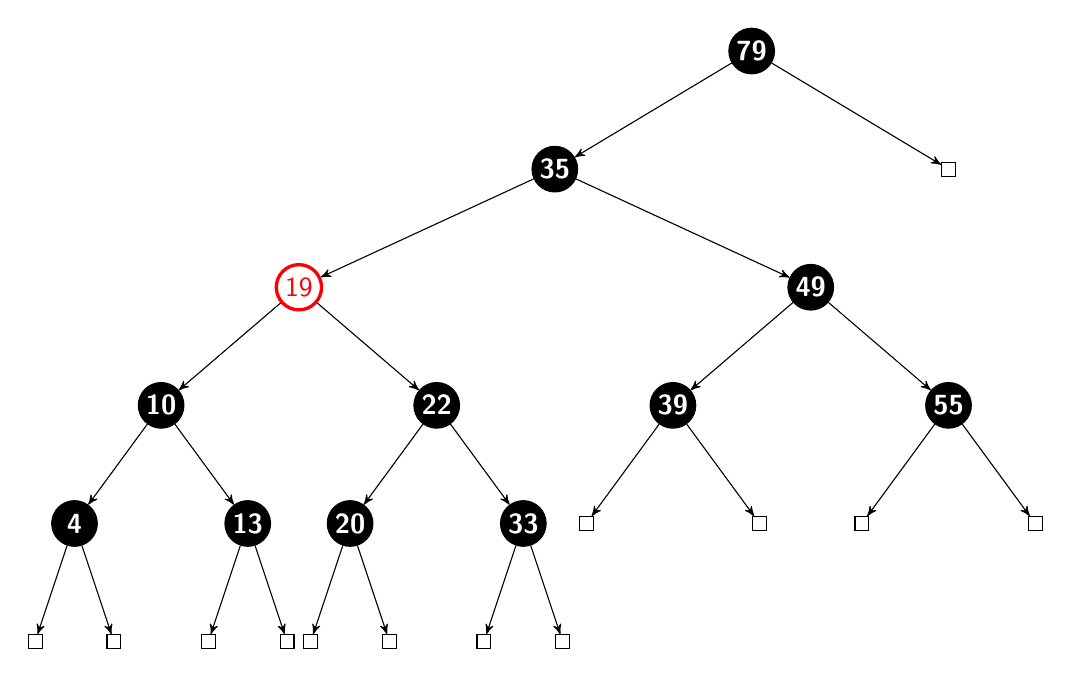
\begin{tikzpicture}[->,>=stealth',level/.style={sibling distance = 5cm/#1, level distance = 1.5cm},
level 2/.style={sibling distance = 6.5cm},
level 3/.style={sibling distance = 3.5cm},
level 4/.style={sibling distance = 2.2cm}
] 
\node [arn_n] {79}
    child{ node [arn_n] {35}
        child{ node [arn_r] {19} 
            child{ node [arn_n, name=leaf 5] {10}
            	child{ node [arn_n] {4}
					child{ node [arn_x] {}}
					child{ node [arn_x] {}}           		
            		}            	
				child{ node [arn_n] {13}
					child{ node [arn_x] {}}
					child{ node [arn_x] {}}
					}
            	}
            child{ node [arn_n] {22}
				child{ node [arn_n] {20}
					child{ node [arn_x] {}}
					child{ node [arn_x] {}}				
				}
				child{ node [arn_n] {33}
					child{ node [arn_x] {}}
					child{ node [arn_x] {}}		
					}
            	}
        	}
        child{ node [arn_n] {49}
            child{ node [arn_n] {39}
					child{ node [arn_x] {}}
					child{ node [arn_x] {}}
            }
            child{ node [arn_n] {55}
					child{ node [arn_x] {}}
					child{ node [arn_x] {}}            
            }
        }                            
    }
    child{ node [arn_x] {}
    }
; 
\end{tikzpicture}
%%%%%%%%%% Step 1 end %%%%%%%%%%%%%
\linebreak
%%%%%%%%%% Step 2 begin %%%%%%%%%%%%%
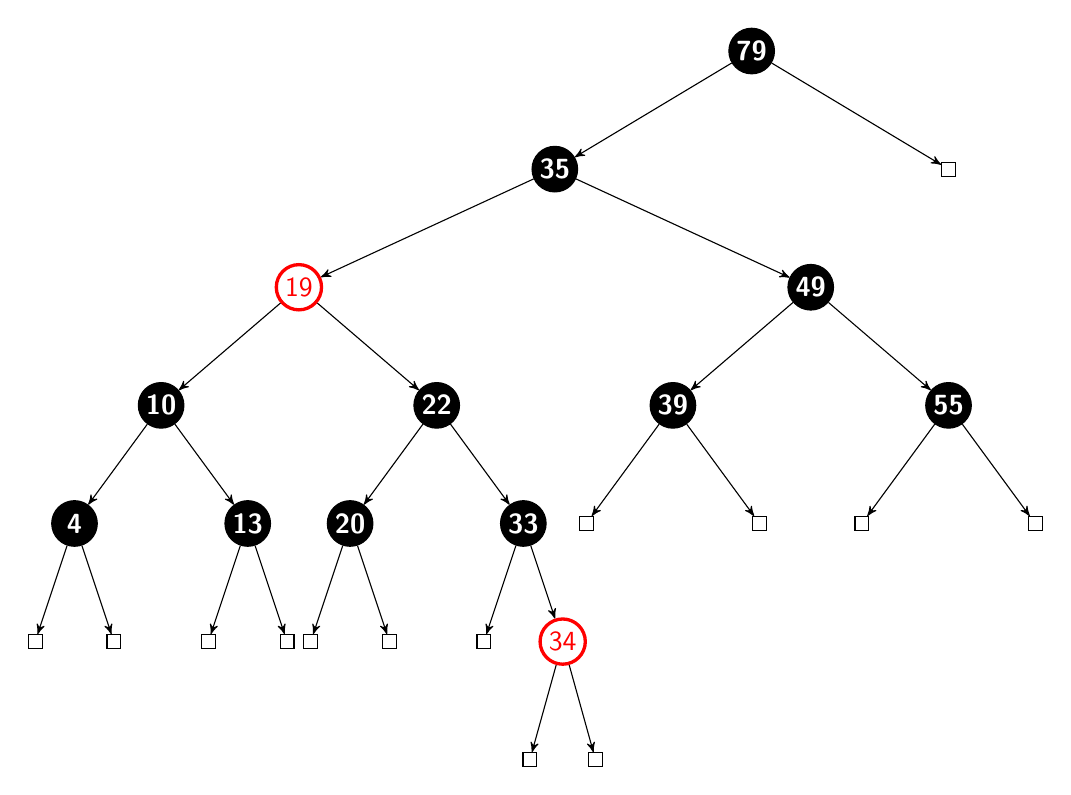
\begin{tikzpicture}[->,>=stealth',level/.style={sibling distance = 5cm/#1, level distance = 1.5cm},
level 2/.style={sibling distance = 6.5cm},
level 3/.style={sibling distance = 3.5cm},
level 4/.style={sibling distance = 2.2cm}
] 
\node [arn_n] {79}
    child{ node [arn_n] {35}
        child{ node [arn_r] {19} 
            child{ node [arn_n, name=leaf 5] {10}
            	child{ node [arn_n] {4}
					child{ node [arn_x] {}}
					child{ node [arn_x] {}}           		
            		}            	
				child{ node [arn_n] {13}
					child{ node [arn_x] {}}
					child{ node [arn_x] {}}
					}
            	}
            child{ node [arn_n] {22}
				child{ node [arn_n] {20}
					child{ node [arn_x] {}}
					child{ node [arn_x] {}}				
				}
				child{ node [arn_n] {33}
					child{ node [arn_x] {}}
					child{ node [arn_r] {34}
						child{ node [arn_x] {}}
						child{ node [arn_x] {}}						
						}		
					}
            	}
        	}
        child{ node [arn_n] {49}
            child{ node [arn_n] {39}
					child{ node [arn_x] {}}
					child{ node [arn_x] {}}
            }
            child{ node [arn_n] {55}
					child{ node [arn_x] {}}
					child{ node [arn_x] {}}            
            }
        }                            
    }
    child{ node [arn_x] {}
    }
; 
\end{tikzpicture}
%%%%%%%%%% Step 2 end %%%%%%%%%%%%%

\section*{Problem 4}
We propose a data structure where we augment to every node of the exiting tree another value which is the pointer to the predecessor of the node. Now for this data structure we will be able to maintain the log (n) time complexity for Insert, Delete and Query operations and yet find the required \textit{k} predecessor in  O (k + log (n)). Although for this we shall have to change the Insert and Delete operations a bit. The details for the same are as follows.\\
\textbf{The tree}\\
A normal RB tree where each node, in addition to its own value also stores the value of its predecessor. So the structure of each node is like\\
\begin{lstlisting}[label={list:first},caption=Node Structure.]
struct Node{
  int val;
  struct Node *pre;	// Pointer to predecessor
  struct Node *left,*right;  
};
\end{lstlisting}
Now the algorithms\\
\textbf{Algorithm for \textit{k} predecessor}\\
\begin{lstlisting}[label={list:first},caption=k predecessor, mathescape = true]
void k_pred (int num_predecessor,int value_to_search, Node * root)
{
	key $\leftarrow$ value_to_search;
	ptr $\leftarrow$ search (key, root);
	if(ptr == NULL)
		return;
	while (k != 0)
	{
		print(ptr.pre.val);
		ptr $\leftarrow$ ptr.pre;
		k = k - 1;	
	}
}

Node * search (int key, Node * root)
{
	p $\leftarrow$ root;
	while(p != NULL)
	{
		if (p.val == key)
			return p;
		else if (p.val > key)
			p $\leftarrow$ p.left;
		else p $\leftarrow$ p.right;
	}
}
\end{lstlisting}
\textbf{Proof of correctness for \textit{k} predecessor}\\
Since this is an iterative algorithm, after every loop the value that it prints is basically the immediate predecessor of the current node. Now as this loop is called exactly k times and every time the loop updates the current node and prints the immediate predecessor to it. Thus, after k iterations when the loop is finally exited it would have published k predecessors of the given number.
Hence, we can conclude that this algorithm gives the correct outputs at the end of execution.\\
\\
\textbf{Time Complexity for the above algorithm}\\
For each query the search effectively does Binary Search and then returns the pointer to it. Thus its time complexity will be log (n) as is know. Now, each iteration of the loop would take 3 * T(1) time and the loop is executed k times. Hence the total time taken is 3 * k * T(1). Hence, the order would be log (n) + k.\\
\\
\textbf{Changes to Insert function}\\
The only change we need to make in Insert is to search for the predecessor of the inserted value and augment this into the newly inserted node. Now, search for the predecessor shall be of order log (n), insert itself is of order log (n). Hence, insert is still done in O (log (n)).\\
\\
\textbf{Changes to Delete function}\\
In deletion we need to store the predecessor of the deleted node in a temporary variable and then after deletion travel to the successor of the deleted node and change its predecessor from the previous value (equal to the deleted node) to the value stored in the temporary variable.
This too similar to the above case will be done in O (log (n)).
\end{document}
